
\section{Perceiving actors on objects}

How could a robot find human arms and hands in the environment without
any prior knowledge of their appearance?  We could imagine segmenting
any moving objects in the scene, and relying on the heuristic that
hands are often the fastest moving objects around.
Another approach is possible in our situation.  If the robot can
detect when an impact event occurs, it can collect segmentations of the
object that caused the impact.  The set of objects that habitually
trigger the motion of other objects is not a bad operational 
definition of a manipulator, and should include the human hand/arm,
and the robot's own arm.  See Figure~\ref{fig:manipulator}.

\ifverbose

Unconstrained motion in a scene is difficult to parse.  But since the
robot has become familiar with a set of objects through poking, it can
constrain the scenarios in which it may identify the manipulator.  In
particular, fixating a familiar object is a necessary condition for
reliably detecting collision.  Fixation is improved by object recognition
and localization, trained my the previous poking episodes.

May fail for more complex events -- e.g. other motion, shadows cast on
object etc.

When the robot fixates an object that it can reach, it will try to poke it.
This is inhibited if it sees motion around the object, giving a human the
opportunity to poke it instead.

The point of contact detection will still work in this case, since it 
doesn't rely on the manipulator being the robot's own arm.

The frames leading up to the impact are great for detecting the
appearance of the manipulator itself.  And give a strong cue that the
moving object is in fact a manipulator (something used to impact
objects).  See Figure~\ref{fig:manipulator}.

\fi

\begin{figure}[tbh]
  \centerline{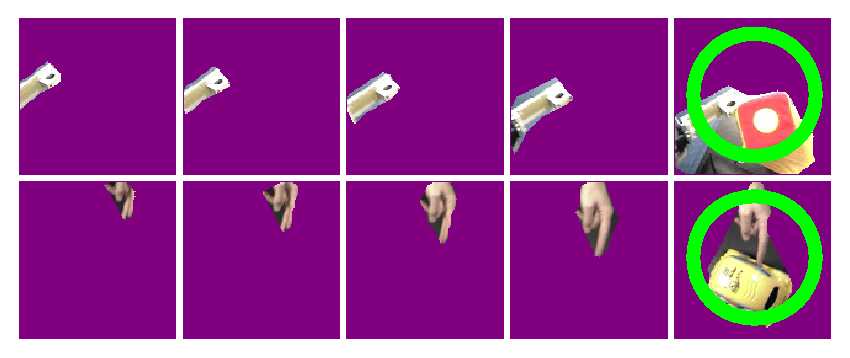
\includegraphics[width=12cm]{manipulator-segment}}
  \caption{Early experiments on segmenting the robot arm, or a 
human hand poking an object the robot is familiar with, by working
backwards from a collision event.}
  \label{fig:manipulator}
\end{figure}

\begin{figure}[tbh]
  \centerline{
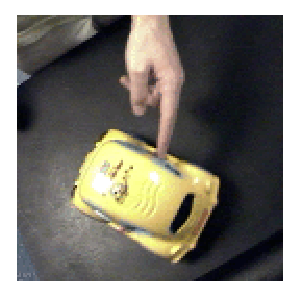
\includegraphics[width=5cm]{fig-car-hand-seg-src}
\hspace{1cm}

\includegraphics[width=5cm]{fig-car-hand-seg}
}
  \caption{A poke by hand}
  \label{fig:handpoke}
\end{figure}

%%Can't necessarily remove shadow.
